% PS_and_IG
\documentclass{standalone}

\usepackage{tikz}
    
\usepackage{graphicx} % Работа с графикой \includegraphics{}
\graphicspath{{./images/img1/}} % картинки в папке ./images/img1/
    
\begin{document}

\begin{tikzpicture}
[line cap=round, line join=round, >=stealth, scale=1]
    % \scriptsize
    \node at (0,0) {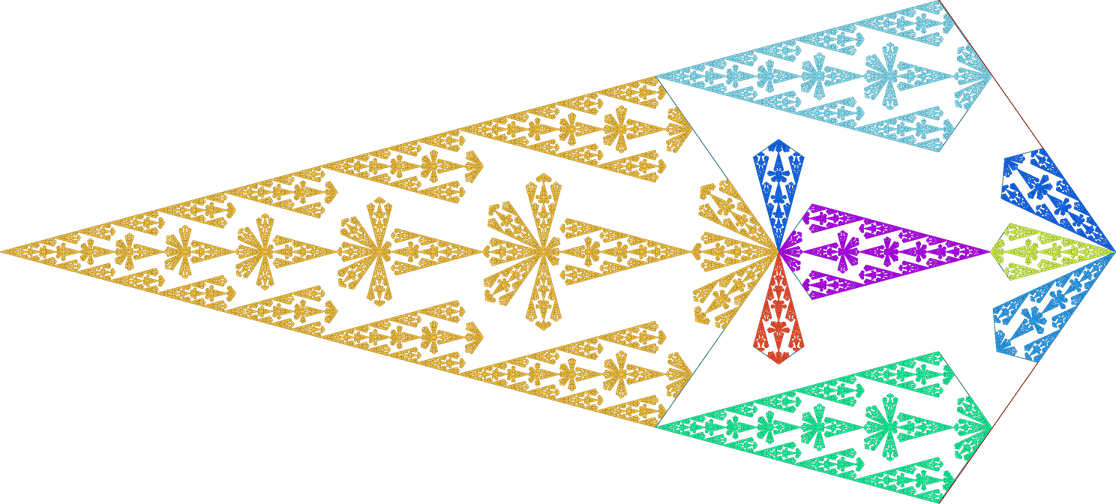
\includegraphics[width=85mm]{rpt6.png}};
    %\draw[help lines] (-4,-3) grid (12,3);
    \node[shape=circle, draw] at (5,0)       (k1) {$K_1$};
    \node[shape=circle, draw] at (5,2)       (k2) {$K_2$};
    \node[shape=circle, draw] at (5,-2)      (k3) {$K_3$};
    \node[shape=circle, draw] at (8,0)       (k4) {$K_4$};
    \node[shape=circle, draw] at (6.5,1.5)   (k5) {$K_5$};
    \node[shape=circle, draw] at (6.5,-1.5)  (k6) {$K_6$};
    \node[shape=circle, draw] at (10,0)      (k7) {$K_7$};
    \node[shape=circle, draw] at (11.5,1.5)  (k8) {$K_8$};
    \node[shape=circle, draw] at (11.5,-1.5) (k9) {$K_9$};
    \draw[fill=black] 
        (5,1)    circle (0.13) 
        (5,-1)   circle (0.13) 
        (6.5,0)  circle (0.13) 
        (9,0)    circle (0.13) 
        (11.5,0) circle (0.13);
    \path[line width=1pt] 
        (k1) edge (k2) 
             edge (k3) 
             edge (k4)
        (k5) edge (k6)
        (k4) edge (k7)
        (11.5,0) edge (k8) 
                 edge (k9) 
                 edge (k7);
    \node at (0,0)      {$K_1$};
    \node at (2.5,1.5)  {$K_2$};
    \node at (2.5,-1.5) {$K_3$};
    \node at (2.7,0.3)  {$K_4$};
    \node at (2.1,0.7)  {$K_5$};
    \node at (2.1,-0.7) {$K_6$};
    \node at (3.6,0)    {$K_7$};
    \node at (4.1,0.6)  {$K_8$};
    \node at (4.1,-0.6) {$K_9$};
\end{tikzpicture}

\end{document}